\documentclass[conference,letterpaper]{IEEEtran}
\usepackage{graphicx}
%\usepackage[dvips]{graphicx}
\usepackage{amsmath}
\usepackage{amssymb}
\usepackage{mathtools} % to typeset small matrices (bsmallmatrix)
\usepackage{calc}
\usepackage{booktabs,hhline} % to typeset table
\usepackage{enumitem}
\usepackage{siunitx}
\usepackage{todonotes}
\usepackage[english]{babel}
%\usepackage[latin1]{inputenc}
\usepackage{url}
\usepackage{algorithm2e}
%----------------------------------
% set algorithm2e styles
%----------------------------------
% change algorithm font size
\SetAlFnt{\footnotesize}

% change algorithm caption style
\newcommand{\xAlCapSty}[1]{\small\sffamily\bfseries\MakeUppercase{#1}}
\SetAlCapSty{xAlCapSty}

% comment style (algorithms)
%\newcommand{\xCommentSty}[1]{\scriptsize\ttfamily\textcolor{blue}{#1}}
%\SetCommentSty{xCommentSty}

% change line number style
%\newcommand\mynlfont[1]{\scriptsize\sffamily{#1}}
%\SetNlSty{mynlfont}{}{} 

% don't print semicolon
\DontPrintSemicolon

% ruled algorithm
\RestyleAlgo{algoruled}

\makeatletter
\newcommand{\removelatexerror}{\let\@latex@error\@gobble}
\makeatother

% If you use a LaTeX that does not use vector fonts by default (e.g., MiKTeX),
% uncomment the following line.
\usepackage{times}
%\let\Bbbk\relax
%\usepackage[subscriptcorrection,slantedGreek,nofontinfo,mtphrb,mtpscr,mtpcal]{mtpro2}
  
% Options for blackboard bold fonts [2.9]:
%   mtphrb - holey roman bold        mtpbb - blackboard bold
%   mtphrd - holey roman bold dark   mtpbbd - blackboard bold dark
%   mtphbi - holey bold italic       mtpbbi - blackboard bold italic
  
% Options for alternate character sets [2.6, 2.7]:
%   mtpcal - assigns Math Script to the math alphabets \mathcal and \mathbcal,
%       overwriting the default math calligraphic typeface
%   mtpccal - assigns Math Curly to the math alphabets \mathcal and \mathbcal,
%       overwriting the default math calligraphic typeface
%   mtpscr - assigns Math Script to the new math alphabets \mathscr and \mathbscr,
%       leaving \mathcal unchanged
%   mtpfrak - assigns Math Fraktur to a new math alphabet \mathfrak

%\usepackage{calrsfs}
%\DeclareMathAlphabet{\pazocal}{OMS}{zplm}{m}{n}

%\usepackage{amssymb}
%\usepackage{url}

\usepackage{cite} % Loading the cite package will result in citation numbers being automatically sorted and properly "ranged". i.e., [1], [9], [2], [7], [5], [6] (without using cite.sty) will become: [1], [2], [5]--[7], [9] (using cite.sty)
%\usepackage{stfloats}  % Gives LaTeX2e the ability to do double column
% floats at the bottom of the page as well as the top.
% (e.g., "\begin{figure*}[!b]" is not normally
% possible in LaTeX2e). This is an invasive package
% which rewrites many portions of the LaTeX2e output
% routines. It may not work with other packages that
% modify the LaTeX2e output routine and/or with other
% versions of LaTeX.

% correct bad hyphenation here
%\hyphenation{op-tical net-works semi-conduc-tor IEEEtran}
\usepackage{siunitx} % to typeset seconds
\usepackage{tikz}
\let\Bbbk\relax
%\usepackage[subscriptcorrection,nofontinfo,mtphrb,mtpscr,mtpcal]{mtpro2_fix}
\usetikzlibrary{decorations.markings,shadows.blur,fit,arrows,calc,fadings,positioning,shapes.arrows,shadows,backgrounds,fit}
%%%%%%%%%%%%%%%%%%%%%%%%%%%%%%%%%%%%%%%%%%%%%%%%%%%%%%%%%%%%%%%%%%%%%%%%%%%%%%%%
\tikzstyle{wrlss}=[rectangle,thick,minimum size=1.8cm,draw=gray!80,fill=gray!10,blur shadow     = {shadow blur steps = 15}]
\tikzstyle{mlss}=[rectangle,thick,minimum size=1.8cm,draw=black,fill=white=!90,fill opacity=0.5]
\tikzstyle{wr}=[rectangle,thick,minimum size=1cm,draw=gray!80,fill=gray!20]
\tikzstyle{rr}=[rectangle,thick,minimum size=1cm,draw=gray!80,fill=red!20,blur shadow={shadow blur steps = 15}]
\tikzstyle{yr}=[rectangle,thick,minimum size=1cm,draw=gray!80,fill=yellow!40,blur shadow={shadow blur steps = 15}]
\tikzstyle{pr}=[rectangle,thick,minimum size=1cm,draw=gray!80,fill=purple!60,blur shadow={shadow blur steps = 15}]
\tikzstyle{gr}=[rectangle,thick,minimum size=1cm,draw=gray!80,fill=green!20,blur shadow={shadow blur steps = 15}]
\tikzstyle{grVecArrow} = [decoration={markings,mark=at position 0.2 with {\arrow{triangle 60[reversed,fill=green!20]}}},double distance=1.4pt, shorten <= 5.5pt, preaction = {decorate}, postaction = {draw,line width=1.4pt, green!20,shorten <= 4.5pt},decoration={markings,mark=at position 1 with {\arrow{triangle 60[fill=green!20]}}}, double distance=1.4pt, shorten >= 4.5pt,  preaction = {decorate},  postaction = {draw,line width=1.4pt, green!20,shorten >= 5.3pt}]
\tikzstyle{grVecArrow1} = [decoration={markings,mark=at position 0.07 with {\arrow{triangle 60[reversed,fill=green!20]}}},double distance=1.4pt, shorten <= 5.5pt, preaction = {decorate}, postaction = {draw,line width=1.4pt, green!20,shorten <= 4.5pt},decoration={markings,mark=at position 1 with {\arrow{triangle 60[fill=green!20]}}}, double distance=1.4pt, shorten >= 4.5pt,  preaction = {decorate},  postaction = {draw,line width=1.4pt, green!20,shorten >= 5.3pt}]
\tikzstyle{purVecArrow} = [decoration={markings,mark=at position 0.15 with {\arrow{triangle 60[reversed,fill=purple!20]}}},double distance=1.4pt, shorten <= 5.5pt, preaction = {decorate}, postaction = {draw,line width=1.4pt, purple!20,shorten <= 4.5pt},decoration={markings,mark=at position 1 with {\arrow{triangle 60[fill=purple!20]}}}, double distance=1.4pt, shorten >= 4.5pt,  preaction = {decorate},  postaction = {draw,line width=1.4pt, purple!20,shorten >= 5.3pt}]
\tikzstyle{purVecArrow1} = [decoration={markings,mark=at position 0.1 with {\arrow{triangle 60[reversed,fill=purple!20]}}},double distance=1.4pt, shorten <= 5.5pt, preaction = {decorate}, postaction = {draw,line width=1.4pt, purple!20,shorten <= 4.5pt},decoration={markings,mark=at position 1 with {\arrow{triangle 60[fill=purple!20]}}}, double distance=1.4pt, shorten >= 4.5pt,  preaction = {decorate},  postaction = {draw,line width=1.4pt, purple!20,shorten >= 5.3pt}]
\tikzstyle{whiVecArrow} = [thick,decoration={markings,mark=at position 0.2 with {\arrow[semithick]{triangle 60[reversed,fill=white]}}},double distance=1.4pt, shorten <= 3.4pt, preaction = {decorate}, postaction = {draw,line width=1.4pt, white,shorten <= 4.5pt}, decoration={markings,mark=at position 1 with {\arrow[semithick]{triangle 60[fill=white]}}},  double distance=1.4pt, shorten >= 4.5pt,  preaction = {decorate},  postaction  = {draw,line width=1.4pt, white,shorten >= 5.0pt}]
\tikzstyle{m}=[rectangle,thick,minimum size=1cm,draw=black,fill=white=!90,fill opacity=0.5]
\tikzset{
	sys/.style={rectangle,minimum height=1.1cm,minimum width=2.1cm,draw=gray!40,align=center,fill=blue!7,blur shadow={shadow blur steps = 15}},
	curvedlink/.style={to path={let \p1=(\tikztostart.east), \p2=(\tikztotarget.west),\n1= {abs(\y2-\y1)/4} in (\p1) arc(90:-90:\n1) -- ([yshift=2*\n1]\p2) arc (90:270:\n1)}}
}
\pgfdeclarelayer{back}
\pgfsetlayers{back,main}

\pagestyle{empty}
%\setlength{\topmargin}{1.1cm}
\setlength{\topmargin}{0.0cm}
%\setlength{\oddsidemargin}{-0.24cm}
%\setlength{\evensidemargin}{-0.24cm}
\setlength{\headsep}{0pt}
\setlength{\headheight}{0pt}
\setlength{\textheight}{24cm}
\setlength{\textwidth}{17.2cm}
\setlength{\columnsep}{4mm}

% Bold latin letters
\newcommand{\bfa}{\ensuremath{\mathbf{a}}}
\newcommand{\bfb}{\ensuremath{\mathbf{b}}}
\newcommand{\bfc}{\ensuremath{\mathbf{c}}}
\newcommand{\bfd}{\ensuremath{\mathbf{d}}}
\newcommand{\bfe}{\ensuremath{\mathbf{e}}}
\newcommand{\bff}{\ensuremath{\mathbf{f}}}
\newcommand{\bfg}{\ensuremath{\mathbf{g}}}
\newcommand{\bfh}{\ensuremath{\mathbf{h}}}
\newcommand{\bfi}{\ensuremath{\mathbf{i}}}
\newcommand{\bfj}{\ensuremath{\mathbf{j}}}
\newcommand{\bfk}{\ensuremath{\mathbf{k}}}
\newcommand{\bfl}{\ensuremath{\mathbf{l}}}
\newcommand{\bfm}{\ensuremath{\mathbf{m}}}
\newcommand{\bfn}{\ensuremath{\mathbf{n}}}
\newcommand{\bfo}{\ensuremath{\mathbf{o}}}
\newcommand{\bfp}{\ensuremath{\mathbf{p}}}
\newcommand{\bfq}{\ensuremath{\mathbf{q}}}
\newcommand{\bfr}{\ensuremath{\mathbf{r}}}
\newcommand{\bfs}{\ensuremath{\mathbf{s}}}
\newcommand{\bft}{\ensuremath{\mathbf{t}}}
\newcommand{\bfu}{\ensuremath{\mathbf{u}}}
\newcommand{\bfv}{\ensuremath{\mathbf{v}}}
\newcommand{\bfw}{\ensuremath{\mathbf{w}}}
\newcommand{\bfx}{\ensuremath{\mathbf{x}}}
\newcommand{\bfy}{\ensuremath{\mathbf{y}}}
\newcommand{\bfz}{\ensuremath{\mathbf{z}}}

\newcommand{\bfA}{\ensuremath{\mathbf{A}}}
\newcommand{\bfB}{\ensuremath{\mathbf{B}}}
\newcommand{\bfBu}{\ensuremath{\mathbf{B}_{\mathrm{u}}}}
\newcommand{\bfBd}{\ensuremath{\mathbf{B}_{\mathrm{d}}}}
\newcommand{\bfBf}{\ensuremath{\mathbf{B}_{\mathrm{f}}}}
\newcommand{\bfBw}{\ensuremath{\mathbf{B}_{\mathrm{w}}}}
\newcommand{\bfC}{\ensuremath{\mathbf{C}}}
\newcommand{\bfD}{\ensuremath{\mathbf{D}}}
\newcommand{\hbfD}{\ensuremath{\hat{\mathbf{D}}}}
\newcommand{\bfDu}{\ensuremath{\mathbf{D}_{\mathrm{u}}}}
\newcommand{\bfDv}{\ensuremath{\mathbf{D}_{\mathrm{v}}}}
\newcommand{\bfDd}{\ensuremath{\mathbf{D}_{\mathrm{d}}}}
\newcommand{\bfDf}{\ensuremath{\mathbf{D}_{\mathrm{f}}}}
\newcommand{\bfE}{\ensuremath{\mathbf{E}}}
\newcommand{\bfF}{\ensuremath{\mathbf{F}}}
\newcommand{\bfG}{\ensuremath{\mathbf{G}}}
\newcommand{\bfH}{\ensuremath{\mathbf{H}}}
\newcommand{\bfI}{\ensuremath{\mathbf{I}}}
\newcommand{\bfJ}{\ensuremath{\mathbf{J}}}
\newcommand{\bfK}{\ensuremath{\mathbf{K}}}
\newcommand{\bfL}{\ensuremath{\mathbf{L}}}
\newcommand{\bfM}{\ensuremath{\mathbf{M}}}
\newcommand{\bfN}{\ensuremath{\mathbf{N}}}
\newcommand{\bfO}{\ensuremath{\mathbf{O}}}
\newcommand{\bfP}{\ensuremath{\mathbf{P}}}
\newcommand{\bfPf}{\ensuremath{\mathbf{P}}}
\newcommand{\bfPp}{\ensuremath{\mathbf{P}'}}
\newcommand{\bfQ}{\ensuremath{\mathbf{Q}}}
\newcommand{\bfR}{\ensuremath{\mathbf{R}}}
\newcommand{\bfS}{\ensuremath{\mathbf{S}}}
\newcommand{\bfT}{\ensuremath{\mathbf{T}}}
\newcommand{\bfU}{\ensuremath{\mathbf{U}}}
\newcommand{\bfV}{\ensuremath{\mathbf{V}}}
\newcommand{\bfW}{\ensuremath{\mathbf{W}}}
\newcommand{\bfX}{\ensuremath{\mathbf{X}}}
\newcommand{\bfY}{\ensuremath{\mathbf{Y}}}
\newcommand{\bfZ}{\ensuremath{\mathbf{Z}}}

% Bold latin letters with bar
\newcommand{\bbfx}{\ensuremath{\bar{\mathbf{x}}}}
\newcommand{\bbfy}{\ensuremath{\bar{\mathbf{y}}}}
\newcommand{\bbfz}{\ensuremath{\bar{\mathbf{z}}}}

\newcommand{\bbfA}{\ensuremath{\bar{\mathbf{A}}}}
\newcommand{\bbfG}{\ensuremath{\bar{\mathbf{G}}}}
\newcommand{\bbfI}{\ensuremath{\bar{\mathbf{I}}}}
\newcommand{\bbfZ}{\ensuremath{\bar{\mathbf{Z}}}}

% Bold latin letters with hat
\newcommand{\hbfd}{\ensuremath{\hat{\mathbf{d}}}}
\newcommand{\hbfv}{\ensuremath{\hat{\mathbf{v}}}}
\newcommand{\hbfx}{\ensuremath{\hat{\mathbf{x}}}}
\newcommand{\hbfy}{\ensuremath{\hat{\mathbf{y}}}}
\newcommand{\hbfz}{\ensuremath{\hat{\mathbf{z}}}}


% Bold latin letters with dot
\newcommand{\dbfx}{\ensuremath{\dot{\mathbf{x}}}}

% Bold latin letters with tilde
\newcommand{\tbfx}{\ensuremath{\tilde{\mathbf{x}}}}


\newcommand{\bffu}[1][,k]{\ensuremath{\mathbf{f}_{\mathrm{u}#1}}}
\newcommand{\bffy}[1][,k]{\ensuremath{\mathbf{f}_{\mathrm{y}#1}}}


\newcommand{\Lk}{\ensuremath{L_{k}\left(\bfx_{k},\bfmu_{k},\bfu_{k},\bfd_{k}\right)}}
\newcommand{\Lok}{\ensuremath{L_{k}\left(\bfx_{0}^{k},\bfmu_{0}^{k},\bfu_{0}^{k},\bfd_{0}^{k}\right)}}
\newcommand{\Lkd}{\ensuremath{L_{k}^{\text{d}}\left(\bfmu_{k},\bfd_{k}\right)}}
\newcommand{\Lkds}[1][k]{\ensuremath{L_{#1}^{\text{d}}\left(\mu_{#1},d_{#1}\right)}}
\newcommand{\Lkc}{\ensuremath{L_{k}^{\text{c}}\left(\bfx_{k},\bfu_{k}\right)}}
\newcommand{\Lkcs}{\ensuremath{L_{k}^{\text{c}}\left(x_{k},u_{k}\right)}}
\newcommand{\Lmaxd}{\ensuremath{L_{\mathrm{max}}^{\text{d}}}}
\newcommand{\Lmaxc}{\ensuremath{L_{\mathrm{max}}^{\text{c}}}}
\newcommand{\Ld}{\ensuremath{L^{\text{d}}\left(\mu,d\right)}}
\newcommand{\Lkdparam}[1][d_{k}]{\ensuremath{L^{\mathrm{d}}(\mu_{k},#1)}}

\newcommand{\bfIdent}{\ensuremath{\mathbf{I}}}
\newcommand{\bfZero}{\ensuremath{\mathbf{0}}}
\newcommand{\bfOne}{\ensuremath{\mathbf{1}}}
\newcommand{\hmu}{\ensuremath{\hat{\mu}}}



\newcommand{\sub}[2][S]{\ensuremath{\mathrm{#1}{#2}}}

% Set of natural numbers
\newcommand{\bbN}{\ensuremath{\mathbb{N}}}

% Set of integer numbers
\newcommand{\bbZ}{\ensuremath{\mathbb{Z}}}

% Set of real numbers
\newcommand{\bbR}{\ensuremath{\mathbb{R}}}

% Set of complex numbers
\newcommand{\bbC}{\ensuremath{\mathbb{C}}}

% Set of discrete time steps
\newcommand{\bbT}{\ensuremath{\mathbb{T}}}


% Calligraphic letters
\newcommand{\mcA}{\ensuremath{\mathcal{A}}}
\newcommand{\mcB}{\ensuremath{\mathcal{B}}}
\newcommand{\mcC}{\ensuremath{\mathcal{C}}}
\newcommand{\mcD}{\ensuremath{\mathcal{D}}}
\newcommand{\mcE}{\ensuremath{\mathcal{E}}}
\newcommand{\mcF}{\ensuremath{\mathcal{F}}}
\newcommand{\mcG}{\ensuremath{\mathcal{G}}}
\newcommand{\mcH}{\ensuremath{\mathcal{H}}}
\newcommand{\mcI}{\ensuremath{\mathcal{I}}}
\newcommand{\mcJ}{\ensuremath{\mathcal{J}}}
\newcommand{\mcK}{\ensuremath{\mathcal{K}}}
\newcommand{\mcL}{\ensuremath{\mathcal{L}}}
\newcommand{\mcM}{\ensuremath{\mathcal{M}}}
\newcommand{\mcN}{\ensuremath{\mathcal{N}}}
\newcommand{\mcO}{\ensuremath{\mathcal{O}}}
\newcommand{\mcP}{\ensuremath{\mathcal{P}}}
\newcommand{\mcQ}{\ensuremath{\mathcal{Q}}}
\newcommand{\mcR}{\ensuremath{\mathcal{R}}}
\newcommand{\mcS}{\ensuremath{\mathcal{S}}}
\newcommand{\mcT}{\ensuremath{\mathcal{T}}}
\newcommand{\mcU}{\ensuremath{\mathcal{U}}}
\newcommand{\mcV}{\ensuremath{\mathcal{V}}}
\newcommand{\mcW}{\ensuremath{\mathcal{W}}}
\newcommand{\mcX}{\ensuremath{\mathcal{X}}}
\newcommand{\mcY}{\ensuremath{\mathcal{Y}}}
\newcommand{\mcZ}{\ensuremath{\mathcal{Z}}}

% Math script letters
\newcommand{\mkZ}{\ensuremath{\mathscr{Z}}}
\newcommand{\mkF}{\ensuremath{\mathscr{F}}}

% Definition of math operators
\DeclareMathOperator*{\mean}{E}				% Expectation operator
\DeclareMathOperator*{\cov}{cov}			% Covariance operator
\DeclareMathOperator*{\var}{var}			% Variance operator
\DeclareMathOperator*{\sign}{sign}			% Signum operator
\DeclareMathOperator*{\tr}{tr}				% Trace operator
\DeclareMathOperator*{\rank}{rank}			% Rank operator
\DeclareMathOperator*{\diff}{d}				% Differential operator
\DeclareMathOperator*{\argmin}{arg\,min}	% Argmin operator
\DeclareMathOperator*{\argmax}{arg\,max}	% Argmax operator
\DeclareMathOperator*{\range}{range}		% Range operator
\DeclareMathOperator*{\nullsp}{null}		% Range operator
\DeclareMathOperator*{\vspan}{span}			% Span operator
\DeclareMathOperator*{\dom}{dom}			% Domain oprator operator
\DeclareMathOperator*{\vect}{vec}			% Vectorization operator
\DeclareMathOperator*{\prst}{P}				% Probability operator

\newcommand{\indfun}{\ensuremath{\mathds{1}}} % Indicator function requires \usepackage{dsfont}
\newcommand{\iu}{\ensuremath{i}}        % Imaginary unit
\providecommand{\e}{\ensuremath{e}}        % Euler's number
\providecommand{\norm}[1]{\lVert#1\rVert}
\newcommand{\T}{\ensuremath{\text{T}}} % Transpose
\newcommand{\Ts}{\ensuremath{T_{\mathrm{s}}}}
\newcommand{\qo}{q^{-1}}
\newcommand{\SISO}{\textsf{SISO}}
\newcommand{\MIMO}{\textsf{MIMO}}
\newcommand{\kf}{\ensuremath{k_{\mathrm{f}}}}
\newcommand{\ka}{\ensuremath{k_{\mathrm{a}}}}
\newcommand{\kfh}{\ensuremath{\hat{k}_{\mathrm{f}}}}

% Bold Greek letters
\newcommand{\bfalpha}{\ensuremath{\boldsymbol{\alpha}}}
\newcommand{\bfbeta}{\ensuremath{\boldsymbol{\beta}}}
\newcommand{\bfdelta}{\ensuremath{\boldsymbol{\delta}}}
\newcommand{\bfDelta}{\ensuremath{\boldsymbol{\Delta}}}
\newcommand{\bfmu}{\ensuremath{\boldsymbol{\mu}}}
\newcommand{\bflambda}{\ensuremath{\boldsymbol{\lambda}}}
\newcommand{\bfLambda}{\ensuremath{\boldsymbol{\Lambda}}}
\newcommand{\bfomega}{\ensuremath{\boldsymbol{\omega}}}
\newcommand{\bftau}{\ensuremath{\boldsymbol{\tau}}}
\newcommand{\bftheta}{\ensuremath{\boldsymbol{\theta}}}
\newcommand{\bfrho}{\ensuremath{\boldsymbol{\rho}}}
\newcommand{\bfeta}{\ensuremath{\boldsymbol{\eta}}}
\newcommand{\bfpsi}{\ensuremath{\boldsymbol{\psi}}}
\newcommand{\bfpi}{\ensuremath{\boldsymbol{\pi}}}
\newcommand{\bfnu}{\ensuremath{\boldsymbol{\nu}}}
\newcommand{\bfsigma}{\ensuremath{\boldsymbol{\sigma}}}
\newcommand{\bfgamma}{\ensuremath{\boldsymbol{\gamma}}}
\newcommand{\bfchi}{\ensuremath{\boldsymbol{\chi}}}
\newcommand{\bfOmega}{\ensuremath{\boldsymbol{\Omega}}}
\newcommand{\bfGamma}{\ensuremath{\boldsymbol{\Gamma}}}
\newcommand{\bfSigma}{\ensuremath{\boldsymbol{\Sigma}}}
\newcommand{\bfSigmav}{\ensuremath{\boldsymbol{\Sigma}_{\mathrm{v}}}}
\newcommand{\bfSigmaw}{\ensuremath{\boldsymbol{\Sigma}_{\mathrm{w}}}}
\newcommand{\bfvarphi}{\ensuremath{\boldsymbol{\varphi}}}
\newcommand{\bfphi}{\ensuremath{\boldsymbol{\phi}}}
\newcommand{\bfPhi}{\ensuremath{\boldsymbol{\Phi}}}
\newcommand{\bfepsilon}{\ensuremath{\boldsymbol{\epsilon}}}
\newcommand{\bfxi}{\ensuremath{\boldsymbol{\xi}}}
\newcommand{\bfzeta}{\ensuremath{\boldsymbol{\zeta}}}

% Bold Greek letters with hat
\newcommand{\hbfxi}{\ensuremath{\hat{\boldsymbol{\xi}}}}

% Special symbols
\newcommand{\Ak}{\ensuremath{\bfA_{\mu_{k}}}}
\newcommand{\Bk}{\ensuremath{\bfB_{\mu_{k}}}}
\newcommand{\Ck}{\ensuremath{\bfC_{\mu_{k}}}}
\newcommand{\Gk}{\ensuremath{\bfG_{\mu_{k}}}}
\newcommand{\Hk}{\ensuremath{\bfH_{\mu_{k}}}}

% Software
\RequirePackage{xspace}
\newcommand{\matlab}{\mbox{\textsc{Matlab}}\xspace}
\newcommand{\yalmip}{\mbox{\textsc{Yalmip}}\xspace}
\newcommand{\cplex}{\mbox{\textsc{CPLEX}}\xspace}
\newcommand{\snopt}{\mbox{\textsc{SNOPT}}\xspace}
\newcommand{\bmibnb}{\mbox{\texttt{bmibnb}}\xspace} 
\def\zeroth{\prescript{0\!}{}}
\def\ist{\prescript{1\!}{}}
\def\iind{\prescript{2\!}{}}
\def\iiird{\prescript{3\!}{}}
\def\nth{\prescript{n\!}{}}
\def\ith{\prescript{i\!}{}}
\def\jth{\prescript{j\!}{}}
\def\bnth{\prescript{\bar{n}\!}{}}
\def\Nth{\prescript{N\!}{}}
\def\dec{\text{dec}}
\def\blkdiag{\mathrm{blkdiag}}

\IEEEoverridecommandlockouts % to display thanks command
\begin{document}
\title{Hierarchical Active Fault Diagnosis for Stochastic Large Scale Systems with Coupled Faults
\thanks{This work was supported by  the Czech Science Foundation, project no. GA18-08531S and by the project LO1506 of the Czech Ministry of Education, Youth and Sports.}
} 
\author{\IEEEauthorblockN{O. Straka, I. Pun\v{c}och\'{a}\v{r}}
  \IEEEauthorblockA{Dept. of Cybernetics, %\& \\European Centre of Excellence NTIS \\Faculty of Applied Sciences\\
    Univ. of West Bohemia\\
  Univerzitn\'{i} 8, 306 14 Pilsen, Czech Republic\\ E-mails: $\{$straka30,ivop$\}$@kky.zcu.cz}
}
% make the title area
\maketitle

%\selectlanguage{english}
\begin{abstract}
  The paper deals with the active fault diagnosis of large scale stochastic systems with faults modeled as mutually dependent Markov chains.
  The system is described by multiple models representing fault-free and faulty behavior of the system.
  The aim of the active fault detector in addition to detecting the faults is to excite the system to improve the detection quality.
  The algorithm consists of two stages: the off-line design of the Bellman function providing the optimal excitation and the on-line estimation, which generates the decisions and selects the optimal excitation according to the Bellman function.
  In particular, the paper focuses on the on-line estimation and proposes an algorithm in the hierarchical architecture.
  The local nodes estimate the continuous state of the subsystems, select the optimal excitations and send local likelihoods to the central node.
  The central node generates the decisions and submits the respective model probabilities to the local nodes.
  The performance of the proposed algorithm is validated using a simple numerical example.
\end{abstract}
\noindent
{\bf Keywords: Fault diagnosis; large-scale systems; multiple-model; distributed estimation}
%%%%%%%%%%%%%%%%%%%%%%%%%%%%%%%%%%%%%%%%%%%%%%%%%%%%%%%%%%%%%%%%%%%%%%%%%%%%%%
\section{Introduction}\label{sec:introduction}
%%%%%%%%%%%%%%%%%%%%%%%%%%%%%%%%%%%%%%%%%%%%%%%%%%%%%%%%%%%%%%%%%%%%%%%%%%%%%%
% LSSs
With increasing complexity and integration of systems, traditional identification, estimation, control and fault diagnosis~(FD) methods become highly inefficient or even unusable.
This is primarily caused by the limitations in \emph{computational power} and \emph{communication bandwidth}.
Although the these have advanced enormously since the first attempts to treat large scale systems (LSSs) in the 1970s, the need of specialized methods for LSSs is still urgent.
To that end, in many engineering problems, the LSS are assumed to consist of several interconnected subsystems of various degree of coupling and spatial distribution, which helps to reduce the computational and communication complexity of the developed methods. 

% FD
The massive automation penetration into many areas entails increasing emphasis on safety critical aspects. 
Indeed, the FD algorithms are quite essential components in current automatic control systems~\cite{Severson2015:cp:SAFEPROCESS}. 
They monitor the system behavior and detect anomalies, sensor or actuator faults, and other factors causing sudden changes in the system behavior. 
Ignorance of such changes often results in undesired maintenance or higher operating costs.

% Passive vs Active FD
With respect to an interaction between the monitored system and the FD algorithms, passive and active approaches are recognized. 
The FD algorithms of the \textit{passive} approach simply monitor the system measurable quantities without any further interaction. 
They have been extensively studied over the past decades and are common in the industrial system monitoring~\cite{Simani2003:b,Blanke2016:b}. 
In the last decade, the \textit{active} approach has attracted attention~\cite{Niemann2005:cp:ACC,Raimondo2016:cp:CDC}. 
The FD algorithms of the active approach, in addition to system quantities monitoring, generate an input signal to excite the monitored system. 
As a consequence of a suitable excitation, more information  is obtained, which can help to detect faults that may be challenging to detect using the passive FD\@. A survey of AFD methods has been published recently in~\cite{HeMe:19}.

In~\cite{Puncochar2019:cp:ACC}, a new AFD framework for stochastic LSSs was introduced with three \emph{architectures} -- centralized, decentralized, and distributed. 
The paper assumed perfect measurements of continuous states of all subsystems to be available to the corresponding AFD nodes. 
Unavailability of such perfect measurements was addressed in~\cite{Straka2019:cp:FUSION}, where only noisy indirect measurements were known to individual AFD nodes. 
The proposed AFD algorithms consisted of two stages, i)~the off-line stage, i.e., design of the excitation input and decision generators, and ii)~the on-line stage, i.e., the state estimation and utilization of the designed generators.
To achieve reasonable computational costs of the AFD algorithm, the off-line design in~\cite{Puncochar2019:cp:ACC,Straka2019:cp:FUSION} rested on the decentralized architecture ignoring the coupling among the LSS subsystems. 

A generalization of the algorithms~\cite{Puncochar2019:cp:ACC,Straka2019:cp:FUSION}, where the faults were assumed independent, was recently proposed in~\cite{StraPu:20}.
In~\cite{StraPu:20}, lagged influence of the faults was assumed, i.e.\ occurrence of a fault in the present may affect occurrences of the faults in other subsystems in the future. 
Formally, the generalization admitted conditionally dependent faults.
However, this generalization may be insufficient in some cases as the faults in different subsystems tend to appear simultaneously or even system-wide faults may emerge. 
This behavior can be formally described as dependent faults.
The goal of the paper is to design an AFD algorithm for LSSs with dependent faults.

The paper is structured as follows: 
Section~\ref{sec:afd_problem_formulation} provides a formulation of the AFD problem; its intractable solution by an AFD algorithm with the centralized architecture is given in Section~\ref{sec:centralized_afd}.
The hierarchical AFD algorithm for an LSS with dependent faults is designed in Section~\ref{sec:hierarchical_afd}.
Its performance is illustrated in Section~\ref{sec:numerical_illustration} and Section~\ref{sec:conclusion} concludes the paper.
%%%%%%%%%%%%%%%%%%%%%%%%%%%%%%%%%%%%%%%%%%%%%%%%%%%%%%%%%%%%%%%%%%%%%%%%%%%%%%
\section{AFD Problem Formulation}\label{sec:afd_problem_formulation}
%%%%%%%%%%%%%%%%%%%%%%%%%%%%%%%%%%%%%%%%%%%%%%%%%%%%%%%%%%%%%%%%%%%%%%%%%%%%%%
This section provides the LSS specification together with its decomposition to subsystems and problem formulation for the AFD\@.
%%%%%%%%%%%%%%%%%%%%%%%%%%%%%%%%%%%%%%%%%%%%%%%%%%%%%%%%%%%%%%%%%%%%%%%%%%%%%%%%
\subsection{System specification}\label{sec:system_specification}
%%%%%%%%%%%%%%%%%%%%%%%%%%%%%%%%%%%%%%%%%%%%%%%%%%%%%%%%%%%%%%%%%%%%%%%%%%%%%%%%
Consider an LSS $\Sigma$ described at a time instant $k\in\mcT\triangleq\{0,1,2,\ldots\}$ by the following discrete-time stochastic state-space model
\begin{subequations}\label{ali:LSS}
	\begin{align}
		\Sigma: \quad  \bfx_{k+1} & =\bff(\bfx_k,\bfmu_k,\bfu_k)+\bfF(\bfmu_k)\bfw_k, \label{ali:LSSdynamics} \\
		\bfy_{k} & =\bfh(\bfx_k,\bfmu_k)+\bfH(\bfmu_k)\bfv_k, \label{ali:LSSmeasurement}
	\end{align}
\end{subequations}
where $\bfs_{k} \triangleq [\bfx^{\T}_{k},\bfmu^{\T}_{k}]^{\T} \in \mcS \triangleq \bbR^{D_x} \times \mcM$ is the state of the LSS, $\bfx_k\in\bbR^{D_x}$ is its continuous part, $\bfmu_k\in\mcM$ is its discrete part, $\bfu_{k}\in\mcU\in\bbR^{D_u}$ is the input, $\bfw_k\in\bbR^{D_x}$ is the state noise described by the known probability density function (PDF) $p_{\bfw_k}$, $\bfy_k\in\bbR^{D_y}$ is the output, and $\bfv_k$ is the measurement noise described by the known PDF $p_{\bfv_k}$. 
The functions $\bff: \bbR^{D_x}\times\mcM\times\mcU\mapsto\bbR^{D_x}$, $\bfh: \bbR^{D_x}\times\mcM\mapsto\bbR^{D_y}$, $\bfF: \mcM\mapsto \bbR^{D_x\times D_x}$, and $\bfH: \mcM\mapsto \bbR^{D_y\times D_y}$ are known. 
Each element of the discrete set $\mcM$ represents an index into a set of $M$ possible models that can describe behavior of the LSS $\Sigma$ in the \emph{fault-free} and \emph{faulty} conditions during a sampling period. 
The faulty conditions are expressed by models with changed parameters or structure. 
The evolution of $\bfmu_k$ is assumed to follow a Markov chain with known transition probabilities
\begin{align}
	\Pr(\bfmu_{k+1}\vert\bfmu_{k}). \label{ali:LSStransition}
\end{align}
The initial condition $\bfs_{0}$ is described by the known PDF\footnote{With a slight abuse of terminology, the function $p(\bfs_{k}) = p(\bfx_{k}, \bfmu_{k})$ is called PDF although $\bfmu_{k}$ is a discrete random variable. 
A more formal notation would require use of a cumulative distribution function or the Dirac delta function.} $p(\bfs_{0})$. 
The state and measurement noises are white, mutually independent, and independent of the initial condition $\bfs_{0}$. 
Thus, for any $k\in\mcT$, it holds that\footnote{A variable or a function with the right subscript $i$ and superscript $j$ stands for the whole sequence of variables or functions from the time instant $i$ to $j$ (e.g., $\bfx_{i}^{j} \triangleq [\bfx_{i}^{\T},\bfx_{i+1}^{\T},\ldots,\bfx_{j}^{\T}]^{\T}$).}
\begin{align}\label{ali:independence}
	p(\bfs_{0},\bfw_{0}^{k},\bfv_{0}^{k}) =	p(\bfs_{0})\prod_{i=0}^{k} p_{\bfw_{i}}(\bfw_{i})p_{\bfv_{i}}(\bfv_{i}).
\end{align}
%Both the continuous part of the state $\bfx_k$ and the discrete part of the state $\bfmu_k$ are unknown and can be observed indirectly through $\bfy_k$.

%%%%%%%%%%%%%%%%%%%%%%%%%%%%%%%%%%%%%%%%%%%%%%%%%%%%%%%%%%%%%%%%%%%%%%%%%%%%%%%%
%\subsection{LSS Decomposition} \label{sec:LSSDecomposition}
%%%%%%%%%%%%%%%%%%%%%%%%%%%%%%%%%%%%%%%%%%%%%%%%%%%%%%%%%%%%%%%%%%%%%%%%%%%%%%%%

Since an active fault detector for the LSS $\Sigma$ with a centralized architecture is not computationally tractable, the decentralized or distributed architectures based on a decomposition $\Sigma$ were considered in~\cite{Puncochar2019:cp:ACC,Straka2019:cp:FUSION}. 
This decomposition is illustrated  in Fig.~\ref{fig:LSSDecomposition}. 
The LSS $\Sigma$ consists of $N$ subsystems $\nth{\Sigma},\ n\in\mcN\triangleq\{1,2,\ldots,N\}$ that are coupled through the state but have separate inputs and outputs\footnote{A symbol with the left superscript pertains to the corresponding subsystem (e.g., $\nth{\Sigma}$), whereas a symbol without the left superscript relates to the whole LSS (e.g., $\Sigma$).}. 
Each subsystem $\nth{\Sigma}$ has its own set of possible fault-free and faulty models and it can be described by the following representation
\begin{subequations}
	\label{ali:subsystem}
	\begin{align}
		\nth{\Sigma}:\ \nth{\bfx}_{k+1} & = \nth{\bff} \left(\bfx_{k},\nth{\mu}_{k},\nth{\bfu}_{k} \right) + \nth{\bfF}(\nth{\mu}_k)\nth{\bfw}_k, \label{ali:subsystemDynamics} \\
		\nth{\bfy}_{k} &= \nth{\bfh} \left(\nth{\bfx}_{k},\nth{\mu}_{k}\right) + \nth{\bfH}(\nth{\mu}_k)\nth{\bfv}_k, \label{ali:subsystemObservation}
	\end{align}
\end{subequations}
where $\nth{\bfs}_{k} \triangleq [\nth{\bfx}^{\T}_{k}, \nth{\mu}_{k}]^{\T} \in \nth{\mcS} \triangleq \bbR^{(\nth{D}_x)} \times \nth{\mcM}$ is the \emph{local} state\footnote{Note that $\nth{\bfs}_{k}$ is called \emph{local} state for convenience, even though it is not technically a state of the subsystem due to the coupling.} of the subsystem $\nth{\Sigma}$, $\nth{\bfx}_{k}\in\bbR^{\nth{D}_x}$ is its continuous part, $\nth{\mu}_{k}\in\nth{\mcM}\triangleq\{1,2,\ldots,\nth{M}\}$ is its discrete part that represents an index into the set of fault-free and faulty models, $\nth{\bfu}_k\in\nth{\mcU}\in\bbR^{\nth{D}_u}$ is the local input, $\nth{\bfw}_k\in\bbR^{\nth{D}_x}$ is the local state noise described by $p_{\nth{\bfw}_k}$, $\nth{\bfy}_k\in\bbR^{\nth{D}_y}$ is the local output, $\nth{\bfv}_k\in\bbR^{\nth{D}_y}$ is the local measurement noise described by $p_{\nth{\bfv}_k}$. 
The functions $\nth{\bff}:\bbR^{D_{x}} \times \nth{\mcM} \times \nth{\mcU} \mapsto \bbR^{\nth{D}_{x}}$, $\nth{\bfh}:\bbR^{\nth{D}_{x}} \times \nth{\mcM} \mapsto \bbR^{\nth{D}_{y}}$, $\nth{\bfF}:\nth{\mcM}\mapsto \bbR^{\nth{D}_{x} \times \nth{D}_{x}}$, and $\nth{\bfH}:\nth{\mcM} \mapsto \bbR^{\nth{D}_{y} \times \nth{D}_{y}}$ are known. 
The set of models $\nth{\mcM}$ includes one model representing the behavior of subsystem $\nth{\Sigma}$ in \emph{fault-free} condition, $\nth{\mu}_{k}=1$, and $\nth{M}-1$ models that represent the behavior of subsystem in \emph{faulty} conditions, $\nth{\mu}_{k}\in\{2,\ldots,\nth{M}\}$.  
% The variables pertaining to \eqref{ali:LSS} and \eqref{ali:subsystem} are related as $\bfx_{k}\triangleq[\ist{\bfx}_{k},\ldots,\Nth{\bfx}_{k}]^{\T}$, $\bfmu_k\triangleq[\ist{\mu}_k,\ldots,\Nth{\mu}_k]^{\T}$, $\bfu_{k}\triangleq[\ist{\bfu}_{k}^{\T},\ldots,\Nth{\bfu}_{k}^{\T}]^{\T}$, $\bfw_{k}\triangleq[\ist{\bfw}_{k}^{\T},\ldots,\Nth{\bfw}_{k}^{\T}]^{\T}$, $\bfy_{k}\triangleq[\ist{\bfy}_{k}^{\T},\ldots,\Nth{\bfy}_{k}^{\T}]^{\T}$, $\bfv_{k}\triangleq[\ist{\bfv}_{k}^{\T},\ldots,\Nth{\bfv}_{k}^{\T}]^{\T}$, $\mcM\triangleq\ist{\mcM}\times\ldots\times\Nth{\mcM}$, $\mcU\triangleq\ist{\mcU}\times\ldots\times\Nth{\mcU}$, $D_x\triangleq\sum_{n=1}^N \nth{D}_x$, $D_{u}\triangleq\sum_{n=1}^{N}\nth{D}_{u}$, $M=\prod_{n=1}^{N}\nth{M}$, $D_y\triangleq\sum_{n=1}^N \nth{D}_y$.
The subsystems are coupled i)~through $\bfx_k$ that appears in the dynamics~\eqref{ali:subsystemDynamics} of all subsystems and ii)~through the multi-model index~$\bfmu_k$ governed by \eqref{ali:LSStransition}.
%The LSS $\Sigma$ given by~\eqref{ali:LSSDecomposition} is assumed to satisfy the following independence condition:


The assumption of complete or conditional independence for $\bfmu_{k}$ among subsystems was made in  \cite{Puncochar2019:cp:ACC,Straka2019:cp:FUSION,StraPu:20} to simplify non-centralized state estimation using a factorization of the initial condition $\Pr(\bfmu_{0})=\prod_{n=1}^{N}\Pr(\nth{\mu}_{0})$ and factorization of the transition probabilities into a product of marginal probabilities
\begin{align}
	\Pr(\bfmu_{k+1}|\bfmu_{k})=
  \begin{cases}
    \prod_{n=1}^N\Pr(\nth{\mu}_{k+1}|\nth{\mu}_{k}) & \text{(in~\cite{Puncochar2019:cp:ACC},~\cite{Straka2019:cp:FUSION})}\\
                                                    &\text{or}\\
    \prod_{n=1}^N\Pr(\nth{\mu}_{k+1}|\bfmu_{k}) & \text{(in~\cite{StraPu:20})}.
  \end{cases}
\end{align}
In order to consider a broader class of the LSSs that includes systems whose transitions between models are correlated across different subsystems and tend to happen simultaneously, these independence assumptions are completely abandoned in this paper.
Note that considering mutually dependent faults facilitates modeling system-wide faults.

The local state and measurement noises are assumed to be independent across the subsystems
\begin{align} \label{ali:independence2}
	p_{\bfw_{k}}(\bfw_{k}) \!\! = \!\! \prod_{n=1}^{N}p_{\nth{\bfw}_{k}}(\nth{\bfw}_{k}), p_{\bfw_{k}}(\bfw_{k}) \!\! = \!\! \prod_{n=1}^{N}p_{\nth{\bfw}_{k}}(\nth{\bfw}_{k}).
\end{align}
The initial state $\bfs_{0}$ is assumed to satisfy
\begin{align}
	p(\bfs_{0}) = \left(\prod_{n=1}^{N} p_{\nth{\bfx}_{0}}(\nth{\bfx}_{0})\right) \Pr(\bfmu_{0}),
\end{align}
where $p_{\nth{\bfx}_0}$ is a known PDF of the initial continuous part of the local state for subsystem $\nth{\Sigma}$ and $\Pr(\bfmu_{0})$ is the initial distribution of the multi-model index $\bfmu_{0}$. Note that similarly to the transition probabilities for $\bfmu_{k}$, no factorization is admitted by the initial distribution $\Pr(\bfmu_{0})$. The only assumption is that the Markov chain~\eqref{ali:LSStransition} converges to its stationary distribution.


\begin{figure}
	\centering
	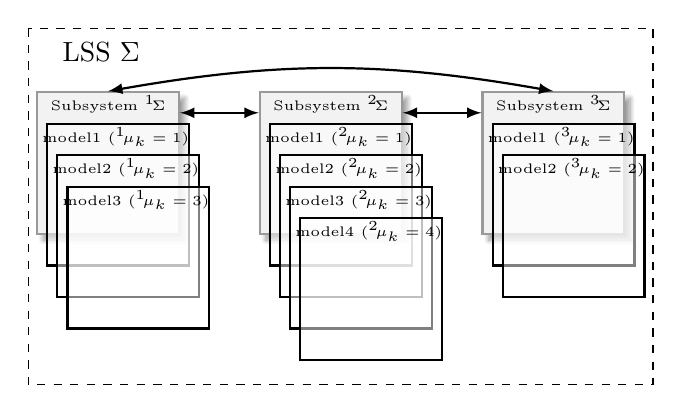
\begin{tikzpicture}
	\node (dix1) [wrlss,label={[yshift=-4.4mm] \tiny Subsystem $\ist{\Sigma}$}] {};
	\node (dix2) [wrlss,right=1.0cm of dix1,label={[yshift=-4.4mm]\tiny Subsystem $\iind{\Sigma}$}] {};
	\node (dix3) [wrlss,right=1.0cm of dix2,label={[yshift=-4.4mm]\tiny Subsystem $\iiird{\Sigma}$}] {};
	\draw[dashed] ($(dix1.north west)+(-.1,0.8)$) rectangle ($(dix3.south east)+(0.35,-1.9)$);
	\node (ldi) at ($(dix1.north east)+(-1,.5)$) {LSS $\Sigma$};
	\draw[latex-latex,thick] (dix1.35) -- (dix2.145);
	\draw[latex-latex,thick] (dix2.35) -- (dix3.145);
	\draw[latex-latex,thick] (dix1.north) to [out=10,in=170]  (dix3.north);
	\node (m11) [mlss,right=-17mm of dix1,yshift=-4mm,label={[yshift=-4.4mm,xshift=-.3mm]\tiny model1 ($\ist{\mu}_k=1$)}]  {};
	\node (m12) [mlss,right=-17mm of m11,yshift=-4mm,label={[yshift=-4.4mm,xshift=-.3mm]\tiny model2 ($\ist{\mu}_k=2$)}]  {};
	\node (m13) [mlss,right=-17mm of m12,yshift=-4mm,label={[yshift=-4.4mm,xshift=-.3mm]\tiny model3 ($\ist{\mu}_k=3$)}]  {};
	\node (m21) [mlss,right=-17mm of dix2,yshift=-4mm,label={[yshift=-4.4mm,xshift=-.3mm]\tiny model1 ($\iind{\mu}_k=1$)}]  {};
	\node (m22) [mlss,right=-17mm of m21,yshift=-4mm,label={[yshift=-4.4mm,xshift=-.3mm]\tiny model2 ($\iind{\mu}_k=2$)}]  {};
	\node (m23) [mlss,right=-17mm of m22,yshift=-4mm,label={[yshift=-4.4mm,xshift=-.3mm]\tiny model3 ($\iind{\mu}_k=3$)}]  {};
	\node (m24) [mlss,right=-17mm of m23,yshift=-4mm,label={[yshift=-4.4mm,xshift=-.3mm]\tiny model4 ($\iind{\mu}_k=4$)}]  {};
	\node (m31) [mlss,right=-17mm of dix3,yshift=-4mm,label={[yshift=-4.4mm,xshift=-.3mm]\tiny model1 ($\iiird{\mu}_k=1$)}]  {};
	\node (m32) [mlss,right=-17mm of m31,yshift=-4mm,label={[yshift=-4.4mm,xshift=-.3mm]\tiny model2 ($\iiird{\mu}_k=2$)}]  {};
	\end{tikzpicture}
	\caption{The decomposition of an LSS into subsystems.}
	\label{fig:LSSDecomposition}
\end{figure}


%%%%%%%%%%%%%%%%%%%%%%%%%%%%%%%%%%%%%%%%%%%%%%%%%%%%%%%%%%%%%%%%%%%%%%%%%%%%%%%%
\subsection{AFD Problem Formulation}\label{sec:AFD_problem_formulation}
%%%%%%%%%%%%%%%%%%%%%%%%%%%%%%%%%%%%%%%%%%%%%%%%%%%%%%%%%%%%%%%%%%%%%%%%%%%%%%%%
The AFD aims to design functions that transform the complete available information to a decision about the faults (subsystem models) and to an input, the role of which is to excite the system to improve the detection quality. 
The active fault detector~$\Delta$ can be described at a time instant $k\in\mcT$ as
\begin{align}\label{ali:AFDsystem}
  \Delta:\quad
  \begin{bmatrix}
    \bfd_{k}\\ \bfu_{k}
  \end{bmatrix} = 
  \bfrho_{k}\left(\bfI_{0}^{k}\right) =
  \begin{bmatrix}
    \bfsigma_{k}\left( \bfI_0^k\right)\\ \bfgamma_{k}\left(\bfI_{0}^{k}\right)
  \end{bmatrix},
\end{align}
where $\bfI_0^k\triangleq[(\bfy_{0}^{k})^{\T},(\bfu_{0}^{k-1})^{\T}]^{\T}\in\mcI^k$ denotes complete available information observed up to the time step $k\in\mcT$ with $\mcI^{k}\triangleq\bbR^{(k+1)D_y}\times\mcU^{k}$ and $\mcU^{k}\triangleq\mcU\times\ldots\times\mcU$. 
The vector $\bfd_{k}\triangleq[\ist{d}_k,\iind{d}_k,\ldots,\Nth{d}_k]^{\T}\in\mcM$ consists of the  decisions $\nth{d}_k\in\nth{\mcM}$ about the model indices~$\nth{\mu}_k$, $\bfsigma_{k}:\mcI^{k} \mapsto \mcM$ represents the fault detector at the time step $k$, and $\bfgamma_{k}:\mcI^{k} \mapsto \mcU$ is a function describing the input signal generator. 

The optimal active fault detector minimizes the following additive discounted criterion\footnote{The operator $\mean\{\cdot\}$ denotes the expectation over all involved random variables.}
\begin{align} \label{ali:criterion}
	J = \lim_{F\to\infty} \mean \left\{ \sum_{k=0}^{F} \eta^{k} L^{\mathrm{d}}(\bfmu_{k},\bfd_{k})\right\},
\end{align}
where $\eta\in(0,1)$ is a chosen discount factor and $L^{\mathrm{d}}:\mcM\times\mcM\mapsto\bbR^{+}$ is a detection cost function that allows different costs to be assigned for selecting the vector of decisions $\bfd_{k}$ when the vector of model indices $\bfmu_{k}$ is actually effective.
This paper assumes that the costs are not related across the subsystems, and thus the following additive detection cost function is used
\begin{align}
	L^{\mathrm{d}}(\bfmu_{k},\bfd_{k}) = \sum_{n=1}^{N} \nth{L}^{\mathrm{d}} \left(\nth{\mu}_{k},\nth{d}_{k} \right), \label{ali:additiveCostFunction}
\end{align}
where $\nth{L}^{\mathrm{d}}:\nth{\mcM}\times\nth{\mcM}\mapsto\bbR^{+}$ is a function that assigns costs to selecting decision $\nth{d}_{k}$ while the true model index is $\nth{\mu}_{k}$. 
The cost function can represent true economic costs of the missed detection, false alarm and, incorrect fault isolation. 
If these costs are not available in a particular problem, they can be regarded as tuning parameters that shape the behavior of the active fault detector~\cite{Puncochar2014:ja:AMCS}.

The basic principles of the design of an AFD algorithm are demonstrated for simplicity using a central architecture.
%%%%%%%%%%%%%%%%%%%%%%%%%%%%%%%%%%%%%%%%%%%%%%%%%%%%%%%%%%%%%%%%%%%%%%%%%%%%%%
\section{Centralized AFD}\label{sec:centralized_afd}
%%%%%%%%%%%%%%%%%%%%%%%%%%%%%%%%%%%%%%%%%%%%%%%%%%%%%%%%%%%%%%%%%%%%%%%%%%%%%%
%%%%%%%%%%%%%%%%%%%%%%%%%%%%%%%%%%%%%%%%%%%%%%%%%%%%%%%%%%%%%%%%%%%%%%%%%%%%%%%%
\subsection{Perfect state information model}\label{sec:perfectStateInformationModel}
%%%%%%%%%%%%%%%%%%%%%%%%%%%%%%%%%%%%%%%%%%%%%%%%%%%%%%%%%%%%%%%%%%%%%%%%%%%%%%%%
Since the active fault detector has access only to inputs and outputs of the LSS but not to its state, the formulated problem belongs to the class of imperfect state information problems~\cite{Bertsekas2012:b}. 
These problems are usually solved by reformulating them as perfect state information problems. 
The reformulation assumes that the active fault detector can be split into a given state estimator and an unknown mapping that transforms the state estimate to the input and decision. 
Then, the aim is to design only this mapping.

The optimal state estimate represented by the conditional PDF $p(\bfs_{k} \vert \bfI_{0}^{k})$~\cite{BarShalom2001:b} is usually approximated using a finite number of statistics that can be collected into an \emph{information state} $\bfxi_{k}\in\mcG$. 
The time evolution of the information state is then described by the following perfect state information model
\begin{align} \label{ali:PerfectStateInformationModel}
	\bfxi_{k+1} = \bfphi \left(\bfxi_{k},\bfu_{k},\bfy_{k+1} \right),
\end{align}
where $\bfphi: \mcG \times \mcU \times \bbR^{D_y} \mapsto \mcG$ is a function that represents the composition of the state estimator calculating~$\bfxi_k$ and the LSS model~$\Sigma$. 
The future output $\bfy_{k+1}$ is regarded in this model as a random disturbance described by the conditional PDF $p(\bfy_{k+1} \vert \bfxi_{k},\bfu_{k})$.

%%%%%%%%%%%%%%%%%%%%%%%%%%%%%%%%%%%%%%%%%%%%%%%%%%%%%%%%%%%%%%%%%%%%%%%%%%%%%%%%
\subsection{AFD for perfect state information model}\label{sec:afdPerfectStateInformationModel}
%%%%%%%%%%%%%%%%%%%%%%%%%%%%%%%%%%%%%%%%%%%%%%%%%%%%%%%%%%%%%%%%%%%%%%%%%%%%%%%%
Given the information state $\bfxi_{k}$, it suffices to consider the active fault detector as a time invariant system that is described at a time step $k\in\mcT$ as
\begin{align}
  \Delta:\quad
  \begin{bmatrix}
    \bfd_{k}\\ \bfu_{k}
  \end{bmatrix} =
  \begin{bmatrix}
    \bar{\bfsigma}(\bfxi_{k})\\ \bar{\bfgamma}(\bfxi_{k})
  \end{bmatrix},
\end{align}
where $\bar{\bfsigma}:\mcG\mapsto\mcM$ and $\bar{\bfgamma}:\mcG\mapsto\mcU$ are unknown functions. 
The detection cost function for the perfect state information model equivalent to $L^{\mathrm{d}}$ in~\eqref{ali:criterion} can be shown~\cite{Puncochar2014:ja:AMCS} to satisfy 
\begin{align}\label{ali:detection_cost_function}
  \bar{L}^{\mathrm{d}}(\bfxi_{k},\bfd_{k}) = 
    \sum_{n=1}^N\sum_{\nth{\mu}_{k}}
    \nth{L}^{\mathrm{d}}(\nth{\mu}_{k},\nth{d}_{k})\Pr(\nth{\mu}_{k} \vert \bfI_{0}^{k}).
\end{align}
Having the reformulated problem specification, the active fault detector is determined by finding a function $V:\mcG\mapsto\bbR$ that solves the Bellman functional equation~\cite{Bertsekas2012:b,Vrabie2013:b}
\begin{multline} \label{ali:BellmanFunctionalEquation}
   V(\bfxi_{k}) = \min_{\bfd'\in\mcM} \bar{L}^{\mathrm{d}}(\bfxi_{k},\bfd')\\
  +\eta\min_{\bfu'\in\mcU} \mean \left\{ V(\bfxi_{k+1}) \vert
  \bfxi_{k},\bfu_k=\bfu' \right\}.
\end{multline}
The Bellman function $V$ can be computed off-line using the a priori known PDF $p ( \bfx_{k+1} \vert \bfx_{k},\bfmu_{k},\bfu_{k} )$, transition probability $\Pr(\bfmu_{k+1} \vert \bfmu_{k})$, measurement PDF $p(\bfy_k\vert \bfx_k,\bfmu_k)$, cost function $L^{\mathrm{d}}$, and discount factor $\eta$. 
Then, the decisions and  inputs can be determined on-line by solving much simpler optimization problems. 
Clearly, the Bellman function $V$ does not need to be known to write the detector as
\begin{align}\label{ali:optimalDecision}
	\bfd_{k} = \bar{\bfsigma}^{*}(\bfxi_{k}) = \argmin_{\bfd'\in\mcM} \bar{L}^{\mathrm{d}}(\bfxi_{k},\bfd').
\end{align}
Note that the detector is determined by the choice of the detection cost function~\eqref{ali:additiveCostFunction}. 
On the other hand, the input signal generator uses the Bellman function $V$ to calculate the input $\bfu_k$ as
\begin{align}\label{ali:optimalInput}
	\bfu_{k} = \bar{\bfgamma}^{*}(\bfxi_{k}) = 	\argmin_{\bfu'\in\mcU} \mean \left\{ V \left( \bfxi_{k+1}\right) \vert \bfxi_{k},\bfu_k=\bfu' \right\}.
\end{align}
Thus, the optimal input generator works in a feedback manner to improve the detection quality.  
%%%%%%%%%%%%%%%%%%%%%%%%%%%%%%%%%%%%%%%%%%%%%%%%%%%%%%%%%%%%%%%%%%%%%%%%%%%%%%%%
%%%%%%%%%%%%%%%%%%%%%%%%%%%%%%%%%%%%%%%%%%%%%%%%%%%%%%%%%%%%%%%%%%%%%%%%%%%%%%
\section{Hierarchical AFD}\label{sec:hierarchical_afd}
%%%%%%%%%%%%%%%%%%%%%%%%%%%%%%%%%%%%%%%%%%%%%%%%%%%%%%%%%%%%%%%%%%%%%%%%%%%%%%
The costs of the Bellman function $V$  computation are extreme for LSSs as the dimension of the information state $\bfxi_{k}$ can be high due to the dimension of the space~$\bbR^{D_x}$  of the continuous part of the state $\bfx_k$ itself, the form of the sufficient statistics\footnote{Depending on the state estimation algorithm, the sufficient statistics may be represented by e.g., conditional mean and covariance matrix of $\bfx_k$ in case of the Kalman filter  or weighted particles in case of the particle filter.}, and the number of the models~$M$. 
To reduce the computational costs of the off-line design, the AFD algorithms proposed in~\cite{Puncochar2019:cp:ACC,Straka2019:cp:FUSION} considered the decentralized architecture, where the coupling among the subsystems was neglected.
While this may seem a highly approximate solution, it significantly reduces the computational demands tied with the Bellman function computation, because each subsystem is treated separately.
%The Bellman functions are defined for information states $\nth{\bfxi}_k$ of the subsystems with dimensions much smaller than the dimension of $\bfxi_k$.
%Additionally, the Bellman functions for the subsystems can be calculated in parallel as they are mutually independent.
The approximations introduced for the off-line design need not be necessarily applied by the on-line estimation algorithm as illustrated in~\cite{Straka2019:cp:FUSION}, where the distributed architecture was used for the on-line estimation.

Here, the algorithm will be designed in a hierarchical structure, where the nodes relevant to the subsystems communicate with each other and also with a central node. 
The scheme of the hierarchical architecture used for the on-line estimation is depicted in Fig.~\ref{fig:HiAFD}.
\begin{figure}[ht]
  \centering
   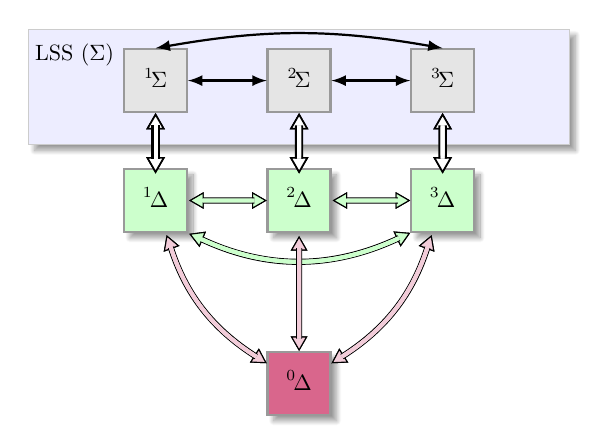
\begin{tikzpicture}[scale=0.8, every node/.style={scale=0.8}]
    \node (dex1) [wr] {$\ist{\Sigma}$};
    \node (dex2) [wr,right=1cm of dex1] {$\iind{\Sigma}$};
    \node (dex3) [wr,right=1cm of dex2] {$\iiird{\Sigma}$};

    \draw[latex-latex,thick] (dex1) -- (dex2);
    \draw[latex-latex,thick] (dex2) -- (dex3);
    \draw[latex-latex,thick] (dex1.north) to [out=10,in=170]  (dex3.north);
    \node (lde) at ($(dex1.north east)+(-1.8,-0.1)$) {LSS ($\Sigma$)};
    \node (defd1) [gr,below=7mm of dex1] {$\ist{\Delta}$};
    \node (defd2) [gr,below=7mm of dex2] {$\iind{\Delta}$};
    \node (defd3) [gr,below=7mm of dex3] {$\iiird{\Delta}$};
    \draw[whiVecArrow] (defd1) -- (dex1);
    \draw[whiVecArrow] (defd2) -- (dex2);
    \draw[whiVecArrow] (defd3) -- (dex3);
    \node (defd0) [pr,below=15mm of defd2] {$\zeroth{\Delta}$};
    \draw[grVecArrow] (defd1) -- (defd2);
    \draw[grVecArrow] (defd2) -- (defd3);
    \draw[grVecArrow1] (defd1.-45) to [out=-25,in=-155] (defd3.-135);
    \draw[purVecArrow1] (defd1) to [bend right=20] (defd0);
    \draw[purVecArrow] (defd2) -- (defd0);
    \draw[purVecArrow1] (defd3) to [bend left=20] (defd0);
    %\draw[-latex,thick] (defd3.-80) to [bend left=20]  (defd0.-10);
    %\draw[-latex,thick] (defd0.10) to [bend right=10]  (defd3.-100);
    %\draw[-latex,thick] (defd1.-80) to [bend right=10]  (defd0.170);
    %\draw[-latex,thick] (defd0.190) to [bend left=20]  (defd1.-100);
    %\draw[-latex,thick] (defd2.-80) to [bend left=5]  (defd0.80);
    %\draw[-latex,thick] (defd0.100) to [bend left=5]  (defd2.-100);
    \begin{pgfonlayer}{back}
      \draw[sys] ($(dex1.north west)+(-1.5,0.3)$) rectangle ($(dex3.south east)+(1.5,-.5)$);
    \end{pgfonlayer}
  \end{tikzpicture}
  \caption{Hierarchical AFD system architecture used for the on-line estimation: the local nodes are in green and the central node is in purple.}\label{fig:HiAFD}
\end{figure}
Based on the calculated estimates, the local nodes will select the optimal excitation input and the central node will generate a decision. 


Thus, the proposed hierarchical AFD for LSS with mutually dependent faults will pursue the following strategy:
i)~The off-line design will employ the computationally efficient decentralized architecture similarly to~\cite{Puncochar2019:cp:ACC,Straka2019:cp:FUSION}.
ii)~The on-line estimation will work in a hierarchical architecture that has the ability to take into account the faults dependency and the coupling through~$\bfx_k$.
%%%%%%%%%%%%%%%%%%%%%%%%%%%%%%%%%%%%%%%%%%%%%%%%%%%%%%%%%%%%%%%%%%%%%%%%%%%%%%
\subsection{Off-line design}\label{sec:off_line_design}
%%%%%%%%%%%%%%%%%%%%%%%%%%%%%%%%%%%%%%%%%%%%%%%%%%%%%%%%%%%%%%%%%%%%%%%%%%%%%%
As has been mentioned above, the off-line design, i.e. the Bellman function calculation, utilizes the decentralized AFD architecture that is depicted in Fig.~\ref{fig:DeAFD}. 
Each subsystem $\nth{\Sigma}$ is monitored by an AFD node $\nth{\Delta}$, which knows only the description of the subsystem $\nth{\Sigma}$, can access only the local output $\nth{\bfy}_k$, and should generate the local input $\nth{\bfu}_{k}$ and decision $\nth{d}_{k}$. 
To achieve such isolation of the AFD nodes, approximate models of subsystems with neglected couplings are needed~\cite{Puncochar2019:cp:ACC}. 
The coupling through $\bfx_{k}$ is neglected by using the following approximate model to describe the subsystem $\nth{\Sigma}$
\begin{subequations}\label{ali:subsystemapprox}
	\begin{align}
		\label{ali:dynamicsapprox}
		\hspace{-1em}\nth{\hat{\Sigma}}:\,
		\nth{\bfx}_{k+1}&=\nth{\hat{\bff}}(\nth{\bfx}_{k},\nth{\mu}_{k},\nth{\bfu}_{k})+\nth{\bfF}(\nth{\mu}_k)\nth{\bfw}_k,\\
		\nth{\bfy}_{k} &= \nth{\bfh} \left(\nth{\bfx}_{k},\nth{\mu}_{k}\right) +
		\nth{\bfH}(\nth{\mu}_k)\nth{\bfv}_k,
	\end{align}
\end{subequations}
where $\nth{\hat{\bff}}:\bbR^{\nth{D}_{x}}\times\nth{\mcM}\times\nth{\mcU}\mapsto\bbR^{\nth{D}_{x}}$ is an approximation of $\nth{\bff}$ obtained by setting $\bnth{\bfx}_{k}=\bfZero$ for $\bar{n}\in\bar{\mcN}\triangleq\mcN\setminus\{n\}$. 
The coupling through the discrete part of the state $\bfmu_{k}$ is neglected in the following way. 
The transition probabilities for the subsystem $\nth{\Sigma}$ can be written as
\begin{align}\label{ali:transitionapprox}
	\Pr(\nth{\mu}_{k+1}|\nth{\mu}_k)=\sum_{\stackrel{\bnth{\mu}_{k+1}}{\bar{n}\in\bar{\mcN}}}\sum_{\stackrel{\bnth{\mu}_k}{\bar{n}\in\bar{\mcN}}}\Pr(\bfmu_{k+1}|\bfmu_k)\frac{\Pr(\bfmu_k)}{\Pr(\nth{\mu}_k)},
\end{align}
where all involved probabilities can be computed using the transition probabilities $\Pr(\bfmu_{k+1}|\bfmu_k)$ and initial probabilities $\Pr(\bfmu_{0})$. 
However, the exact transition probabilities  $\Pr(\nth{\mu}_{k+1}|\nth{\mu}_k)$ are not suitable for designing the AFD node $\nth{\Delta}$ because they are time-varying due to the fraction on the right hand side of~\eqref{ali:transitionapprox}. 
Since the infinite horizon is considered, it seems reasonable to approximate the fraction as
\begin{align}
	\label{ali:coupling_ignorance}
	\frac{\Pr(\bfmu_k)}{\Pr(\nth{\mu}_k)}\approx \lim_{k\to\infty} \frac{\Pr(\bfmu_k)}{\Pr(\nth{\mu}_k)}
\end{align}
provided that the limit exists. 
The design criterion is naturally decomposed by the additive structure of the detection cost function~\eqref{ali:additiveCostFunction} and thus the design criterion for the subsystem $\nth{\Sigma}$ is
\begin{align}
	\nth{J} = \lim_{F\to\infty} \mean \left\{ \sum_{k=0}^{F} \eta^{k} \nth{L}^{\mathrm{d}}(\nth{\mu}_{k},\nth{d}_{k})\right\}.
\end{align}
\begin{figure}[ht]
  \centering
  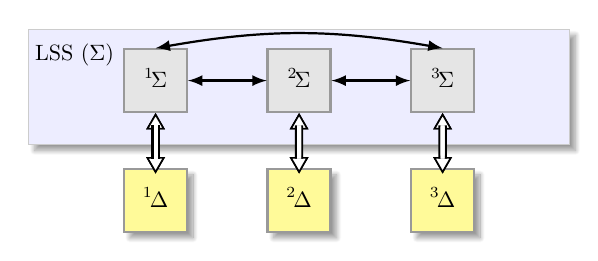
\begin{tikzpicture}[scale=0.8, every node/.style={scale=0.8}]
    \node (dex1) [wr] {$\ist{\Sigma}$};
    \node (dex2) [wr,right=1cm of dex1] {$\iind{\Sigma}$};
    \node (dex3) [wr,right=1cm of dex2] {$\iiird{\Sigma}$};

    \draw[latex-latex,thick] (dex1) -- (dex2);
    \draw[latex-latex,thick] (dex2) -- (dex3);
    \draw[latex-latex,thick] (dex1.north) to [out=10,in=170]  (dex3.north);
    \node (lde) at ($(dex1.north east)+(-1.8,-0.1)$) {LSS ($\Sigma$)};
    \node (defd1) [yr,below=7mm of dex1] {$\ist{\Delta}$};
    \node (defd2) [yr,below=7mm of dex2] {$\iind{\Delta}$};
    \node (defd3) [yr,below=7mm of dex3] {$\iiird{\Delta}$};
    \draw[whiVecArrow] (defd1) -- (dex1);
    \draw[whiVecArrow] (defd2) -- (dex2);
    \draw[whiVecArrow] (defd3) -- (dex3);
\begin{pgfonlayer}{back}
    \draw[sys] ($(dex1.north west)+(-1.5,0.3)$) rectangle
    ($(dex3.south east)+(1.5,-.5)$);
\end{pgfonlayer}
  \end{tikzpicture}
  \caption{Decentralized AFD system architecture used in off-line design}\label{fig:DeAFD}
\end{figure}
The centralized architecture described in Section~\ref{sec:afd_problem_formulation} for the whole LSS can be applied to the individual subsystems separately. 
For each subsystem $\nth{\Sigma}$, the perfect state information model $\nth{\bfphi}:\nth{\mcG} \times \nth{\mcU} \times \bbR^{\nth{D}_y} \mapsto \nth{\mcG}$ with an information state $\nth{\bfxi}_{k}\in\nth{\mcG}$ is built using its approximate model and the Bellman function $\nth{V}$ is computed. 
The numerical computation of the Bellman functions for all subsystems is less demanding because it can be performed in parallel and the information states $\nth{\bfxi}_{k}$ have smaller dimensions compared to $\bfxi_{k}$. 
The AFD node $\nth{\Delta}$ is then defined as
\begin{align}\label{ali:DeAFD}
	\nth{\Delta}:
	\begin{bmatrix}
		\nth{d}_{k}\\
		\nth{\bfu}_{k}
	\end{bmatrix} =% \bfrho_{k}^{\dec} \left( \nth{\bfx}_{0}^{k},\nth{\bfu}_{0}^{k-1} \right) =
	\begin{bmatrix}
		\nth{\bar{\sigma}}^{*} \left( \nth{\bfxi}_{k} \right)\\
		\nth{\bar{\bfgamma}}^{*} \left( \nth{\bfxi}_{k} \right)
	\end{bmatrix},
\end{align} 
where $\nth{\bar{\sigma}}^{*}:\nth{\mcG}\mapsto\nth{\mcM}$ and $\nth{\bar{\bfgamma}}^{*}:\nth{\mcG} \mapsto \nth{\mcU}$ are given by relations similar to~\eqref{ali:optimalDecision} and~\eqref{ali:optimalInput}, respectively. 
The input signal generator $\nth{\bar{\bfgamma}}^{*}$ is kept at each AFD node to generate the input $\nth{\bfu}_{k}$ based on the information state $\nth{\bfxi}_{k}$. 
The decision generator $\nth{\bar{\sigma}}^{*}$ will be moved to the central node of the hierarchical architecture and will use an information state of a better quality. 
If the hierarchical architecture is used for the off-line design, the computational demands will become intractable similarly to the centralized architecture. 
Note that the input generator $\nth{\bar{\bfgamma}}^{*}$ is thus an approximation for the following reasons: approximate model of the subsystem is used,approximate Bellman function is computed numerically, and hierarchical architecture for decision generation is used instead of the decentralized one. 
%%%%%%%%%%%%%%%%%%%%%%%%%%%%%%%%%%%%%%%%%%%%%%%%%%%%%%%%%%%%%%%%%%%%%%%%%%%%%%
\subsection{On-line estimation}\label{sec:on_line_estimation}
%%%%%%%%%%%%%%%%%%%%%%%%%%%%%%%%%%%%%%%%%%%%%%%%%%%%%%%%%%%%%%%%%%%%%%%%%%%%%%
To utilize all available information, the on-line estimation must deal with two couplings present in the LSS $\Sigma$: i)~the coupling in the continuous state $\bfx_k$ and ii)~the coupling in the multi-model index $\bfmu_k$.
While the coupling in $\bfx_k$ will be dealt with by the communication among the local nodes $\nth{\Delta},\ n=1,\ldots,N$ similarly to the distributed architecture~\cite{Straka2019:cp:FUSION}, the coupling in $\bfmu_k$ will be resolved by the communication of the local nodes with a central node denoted as $\zeroth{\Delta}$.
%%%%%%%%%%%%%%%%%%%%%%%%%%%%%%%%%%%%%%%%%%%%%%%%%%%%%%%%%%%%%%%%%%%%%%%%%%%%%%
\subsubsection{Local nodes}\label{sec:local_nodes}
%%%%%%%%%%%%%%%%%%%%%%%%%%%%%%%%%%%%%%%%%%%%%%%%%%%%%%%%%%%%%%%%%%%%%%%%%%%%%%
The part of the on-line estimation performed by the local nodes consists of the information exchange with the central node, measurement update, merging, information exchange with other local nodes, information fusion, selection of the optimal excitation input signal, and time update steps. Their brief description for the $n$-th node $\nth{\Delta}$ follows.

\textbf{Assume:} The prediction PDFs of the local continuous state $p(\nth{\bfx}_{k}\vert\nth{\bfI}^{k-1}_{0},\nth{\bfu}_{k-1},\nth{\mu}_{k-1})$ are given for each model $\nth{\mu}_{k-1}\in\nth{\mcM}$, where $\nth{\bfI}_0^k\triangleq[(\nth{\bfy}_{0}^{k})^{\T},(\nth{\bfu}_{0}^{k-1})^{\T}]^{\T}\in\nth{\mcI}^k$ denotes the local data observed up to time step $k \in \mcT$ by the $n$-th AFD node with $\nth{\mcI}^{k}\triangleq\bbR^{(k+1)(\nth{D}_y)}\times\nth{\mcU}^{k}$, $\nth{\mcU}^{k}\triangleq\nth{\mcU}\times\ldots\times\nth{\mcU}$.\\
\textbf{Communication with $\zeroth{\Delta}$:} The likelihoods for each combination of models $\nth{\mu}_{k-1}$ and $\nth{\mu}_k$ calculated as\footnote{Note that the PDF $p\left(\nth{\bfy}_{k}\vert\nth{\bfx}_{k},\nth{\mu}_k\right)$ is obtained from~\eqref{ali:subsystemObservation} and the measurement noise PDF~$p_{\nth{\bfv}_k}$.}
\begin{multline*}
  p(\nth{\bfy}_k\vert\nth{\bfI}_0^{k-1},\nth{\bfu}_{k-1},\nth{\mu}_k,\nth{\mu}_{k-1})=\\
  \int p\left(\nth{\bfy}_{k} \vert\nth{\bfx}_{k},\nth{\mu}_k\right) 
  p\left(\nth{\bfx}_{k}\vert
  \nth{\bfI}^{k-1}_{0},\nth{\bfu}_{k-1},\nth{\mu}_{k-1}\right)d\nth{\bfx}_k,
 \end{multline*}
are sent to the central node $\zeroth{\Delta}$, and processed there.
Then, the probabilities\footnote{Note that the probabilities are conditioned by the full information $\bfI_0^k$ as the central node computes them using likelihoods from all local nodes.} $\Pr(\nth{\mu}_k,\nth{\mu}_{k-1}|\bfI_0^k)$ are received from $\zeroth{\Delta}$.\\
\textbf{Measurement update:}
The posterior PDF of the local state $p(\nth{\bfs}_{k} \vert\nth{\bfI}^{k}_{0})$ factorized as
\begin{multline}\label{ali:PDF_BRR_Posterior}
  p(\nth{\bfs}_{k} \vert\nth{\bfI}^{k}_{0})=\sum_{\nth{\mu}_{k-1}} 
  p(\nth{\bfx}_{k},\nth{\mu}_k,\nth{\mu}_{k-1} \vert \nth{\bfI}^{k}_{0})
  \\=\sum_{\nth{\mu}_{k-1}}
  p(\nth{\bfx}_{k}\vert\nth{\bfI}^{k}_{0},\nth{\mu}_k,\nth{\mu}_{k-1})
  \Pr(\nth{\mu}_k,\nth{\mu}_{k-1} \vert \bfI^{k}_{0} ),
\end{multline}
is obtained by combining the probabilities $\Pr(\nth{\mu}_k,\nth{\mu}_{k-1} \vert \bfI^{k}_{0})$ received from~$\zeroth{\Delta}$ and the PDFs of $\nth{\bfx}_k$ inferred by the Bayes rule
\begin{multline*}
  p(\nth{\bfx}_{k}\vert\nth{\bfI}^{k}_{0},\nth{\mu}_k,\nth{\mu}_{k-1})
  =\\ \frac{p\left(\nth{\bfy}_{k} \vert\nth{\bfx}_{k},\nth{\mu}_k\right) 
  p\left(\nth{\bfx}_{k}\vert \nth{\bfI}^{k-1}_{0},\nth{\bfu}_{k-1},\nth{\mu}_{k-1}\right)}
  {p(\nth{\bfy}_k\vert\nth{\bfI}_0^{k-1},\nth{\bfu}_{k-1},\nth{\mu}_k,\nth{\mu}_{k-1})}.
\end{multline*}  
\textbf{Merging:} The generalized pseudo-Bayesian method of the second order~\cite{Watanabe1993:ja} is used to prevent the increase in the number of terms constituting the state estimate PDF\footnote{Note that at the first time step, the measurement update step is simpler and the merging step is unnecessary.} $p(\nth{\bfs}_{k} \vert\nth{\bfI}^{k}_{0})$. 
Essentially, the sum in the posterior PDF~\eqref{ali:PDF_BRR_Posterior} is merged to a single term for each $\nth{\mu}_k$.
Then, the posterior PDF is approximated by 
\begin{align}\label{ali:posterior}
  p(\nth{\bfs}_{k} \vert\nth{\bfI}^{k}_{0})\approx p(\nth{\bfx}_{k}\vert\nth{\bfI}^{k}_{0},\nth{\mu}_k) \Pr(\nth{\mu}_k\vert \nth{\bfI}^{k}_{0} ).
\end{align}
\textbf{Communication with local nodes:} The $\nth{M}$ PDFs $p(\nth{\bfx}_{k}\vert\nth{\bfI}^{k}_{0},\nth{\mu}_k)$ weighted by $\Pr(\nth{\mu}_k\vert \nth{\bfI}^{k}_{0} )$ are merged to a single PDF denoted as $p(\nth{\bfx}_k\vert\nth{\bfI}^k_0)$ and sent to other local nodes. 
Reciprocally, $\nth{\Delta}$ receives the estimates  $p(\bnth{\bfx}_k\vert\bnth{\bfI}^k_0)$, $\bar{n}\in\bar{\mcN}$ from other local nodes $\bnth{\Delta},\ \bar{n}\in\bar{\mcN}$.\\
\textbf{Fusion:}
The estimates $p(\bnth{\bfx}_k\vert\bnth{\bfI}^k_0)$ are fused with $p(\nth{\bfx}_{k}\vert\nth{\bfI}^{k}_{0},\nth{\mu}_k)$ to obtain $p(\bfx_{k}|\bfI_0^{k},\nth{\mu}_k)$.
The fusion must respect the fact, that the estimates of the local states $\nth{\bfx}_k$, $n\in\mcN$ are dependent but the degree of dependence is unknown. 
For example, if the estimates are represented by the means and covariance matrices, the unknown dependency issue can be solved by the covariance intersection technique~\cite{JuUhl:97}. 
If the estimate is represented by weighted particles, the techniques proposed in e.g.~\cite{Tslil2018:cp:IF} or~\cite{Ajgl2011:cp:IF} can be used.\\
\textbf{Input generation:} The excitation input is computed as $\nth{\bfu}_{k}=\nth{\bar{\bfgamma}}(\nth{\bfxi}_k)$, where $\nth{\bar{\bfgamma}}$ was designed in the off-line design, and the information state $\nth{\bfxi}_k$ is constructed from the estimate~\eqref{ali:posterior}.\\
\textbf{Time update:} The prediction PDFs $p(\nth{\bfx}_{k+1}\vert \bfI^{k}_{0},\nth{\bfu}_{k},\nth{\mu}_{k} )$  are calculated\footnote{Note that the PDF $p \left(\nth{\bfx}_{k+1} \vert \bfx_{k},\nth{\mu}_{k},\nth{\bfu}_{k},\right)$ is obtained from~\eqref{ali:dynamicsapprox} and the state noise PDF $p_{\nth{\bfw}_k}$.} from 
\begin{multline*}
	p(\nth{\bfx}_{k+1} \vert \bfI^{k}_{0}, \nth{\bfu}_{k},\nth{\mu}_{k}) =\\
	\int  p (\nth{\bfx}_{k+1} \vert \bfx_{k}, \nth{\mu}_{k}, \nth{\bfu}_{k} ) p(\bfx_{k} \vert\bfI^{k}_{0},\nth{\mu}_{k})\mathrm{d}\bfx_{k}.
\end{multline*}
%%%%%%%%%%%%%%%%%%%%%%%%%%%%%%%%%%%%%%%%%%%%%%%%%%%%%%%%%%%%%%%%%%%%%%%%%%%%%%
\subsubsection{Central node}\label{sec:central_node}
%%%%%%%%%%%%%%%%%%%%%%%%%%%%%%%%%%%%%%%%%%%%%%%%%%%%%%%%%%%%%%%%%%%%%%%%%%%%%%
The goal of the on-line estimation performed at the central node is to infer the probabilities of the multi-model index $\bfmu_k$ and subsequently the decisions $\nth{d}_k$ from the likelihoods sent by the local nodes. 
Then, the relevant model probabilities are sent back to the local nodes.
Individual steps of the central node are briefly introduced below.\\
\textbf{Assume:} The prediction probabilities $\Pr(\bfmu_{k},\bfmu_{k-1}|\bfI_0^{k-1})$ are given.\\
\textbf{Measurement update:} Once the likelihoods $p(\nth{\bfy}_k\vert\nth{\bfI}_0^{k-1},\nth{\bfu}_{k-1},\nth{\mu}_k,\nth{\mu}_{k-1})$, $n\in\mcN$ are received from the local nodes, the posterior probability of the multi-model indices $\bfmu_k$ and $\bfmu_{k-1}$ are given by 
\begin{multline}\label{ali:Prob_Posterior}
	\Pr(\bfmu_{k},\bfmu_{k-1}|\bfI_0^{k}) \propto\\ \Pr(\bfmu_{k},\bfmu_{k-1}|\bfI_0^{k-1}) p(\bfy_{k}|\bfI_0^{k-1},\bfu_{k-1},\bfmu_{k},\bfmu_{k-1}),
\end{multline}
where  the likelihood is given as
\begin{multline}
	p(\bfy_{k}|\bfI_0^{k-1},\bfu_{k-1},\bfmu_{k},\bfmu_{k-1}) =\\
	\int p\left( \bfy_{k}|\bfx_{k},\bfmu_{k} \right) p\left( \bfx_{k} |\bfI_{0}^{k-1},\bfu_{k-1},\bfmu_{k-1} \right) \mathrm{d}\bfx_{k}.
\end{multline}
Due to the assumption of independent measurement noises~\eqref{ali:independence2}, it is possible to write the conditional PDF $p( \bfy_{k}|\bfx_{k},\bfmu_{k} )$ as
\begin{align}
	p\left( \bfy_{k}|\bfx_{k},\bfmu_{k} \right) = \prod_{n=1}^{N} p\left( \nth{\bfy}_{k}|\nth{\bfx}_{k},\nth{\mu}_{k} \right).
\end{align}
The conditional PDF $p\left( \bfx_{k} |\bfI_{0}^{k-1},\bfu_{k-1},\bfmu_{k-1} \right)$ is approximated by assuming conditional independence as
\begin{multline}
	p\left( \bfx_{k} |\bfI_{0}^{k-1},\bfu_{k-1},\bfmu_{k-1} \right) \approx\\
	\prod_{n=1}^{N} p\left( \nth{\bfx}_{k} | \nth{\bfI}_{0}^{k-1},\nth{\bfu}_{k-1},\nth{\mu}_{k-1} \right).
\end{multline}
Thus, the likelihood in \eqref{ali:Prob_Posterior} is approximated as
\begin{multline} \label{ali:likelihoodApprox}
	p(\bfy_{k}|\bfI_0^{k-1},\bfu_{k-1},\bfmu_{k},\bfmu_{k-1}) \approx\\
	\prod_{n=1}^{N} \int p\left( \nth{\bfy}_{k}|\nth{\bfx}_{k},\nth{\mu}_{k} \right) p\left( \nth{\bfx}_{k} | \nth{\bfI}_{0}^{k-1},\nth{\bfu}_{k-1},\nth{\mu}_{k-1} \right) \mathrm{d}\bfx_{k}\\
	=\prod_{n=1}^{N} p(\nth{\bfy}_k\vert\nth{\bfI}_0^{k-1},\nth{\bfu}_{k-1},\nth{\mu}_k,\nth{\mu}_{k-1}).
\end{multline}
\textbf{Decision generation:} After marginalizing~\eqref{ali:Prob_Posterior}, the conditional probabilities of the model index $\nth{\mu}_{k}$ are used to generate the decisions $\nth{d}_{k}$.\\
\textbf{Communication with local nodes:} The marginal probabilities $\Pr(\nth{\mu}_k,\nth{\mu}_{k-1}|\bfI_0^k)$ are sent to the local AFD nodes.\\
\textbf{Time update:} The predictive probability of the multi-model indices $\bfmu_{k+1}$ and $\bfmu_k$ is calculated as 
\begin{align*}
	\Pr(\bfmu_{k+1},\bfmu_k|\bfI_0^k) = \Pr(\bfmu_{k+1}|\bfmu_k) \sum_{\bfmu_{k-1}} \Pr(\bfmu_k,\bfmu_{k-1}|\bfI_0^k).
\end{align*}
%%%%%%%%%%%%%%%%%%%%%%%%%%%%%%%%%%%%%%%%%%%%%%%%%%%%%%%%%%%%%%%%%%%%%%%%%%%%%%
\subsubsection{Remarks}\label{sec:remarks}
%%%%%%%%%%%%%%%%%%%%%%%%%%%%%%%%%%%%%%%%%%%%%%%%%%%%%%%%%%%%%%%%%%%%%%%%%%%%%%
The proposed AFD with hierarchical architecture consists of two communication layers: i)~the communication among the local nodes, where the nodes exchange the PDFs $p(\nth{\bfx}_k\vert\nth{\bfI}^k_0)$ and ii)~the communication with the central node, where the local nodes submit the likelihoods $p(\nth{\bfy}_k\vert\nth{\bfI}_0^{k-1},\nth{\bfu}_{k-1},\nth{\mu}_k,\nth{\mu}_{k-1})$ and receive the probabilities $\Pr(\nth{\mu}_k,\nth{\mu}_{k-1}|\bfI_0^k)$.
  The optimal decisions $\nth{d}_{k}$ are generated by the central node $\zeroth{\Delta}$ while the excitation input signals $\nth{\bfu}_{k}=\nth{\bar{\bfgamma}}(\nth{\bfxi}_k)$ are generated by the local nodes $\nth{\Delta}$  
%%%%%%%%%%%%%%%%%%%%%%%%%%%%%%%%%%%%%%%%%%%%%%%%%%%%%%%%%%%%%%%%%%%%%%%%%%%%%%
%%%%%%%%%%%%%%%%%%%%%%%%%%%%%%%%%%%%%%%%%%%%%%%%%%%%%%%%%%%%%%%%%%%%%%%%%%%%%%
\section{Numerical Illustrations}\label{sec:numerical_illustration}
%%%%%%%%%%%%%%%%%%%%%%%%%%%%%%%%%%%%%%%%%%%%%%%%%%%%%%%%%%%%%%%%%%%%%%%%%%%%%%
For brevity reasons, the performance of the proposed algorithm is analyzed by means of a simple numerical example only. 
The analysis compares performance of three active fault detectors:
\begin{itemize}
  \item the decentralized AFD algorithm that generates the decisions locally and completely ignores the coupling among the LSS subsystems~\cite{Straka2019:cp:FUSION} (decAFD),
  \item the distributed AFD algorithm that generates the decisions locally and ignores the coupling in $\bfmu_k$ (faults) among the LSS subsystems~\cite{Straka2019:cp:FUSION} (disAFD),
  \item the proposed hierarchical AFD algorithm (hiAFD).
\end{itemize}
\subsection{System specification}
\label{sec:ExampleSystemSpecification}
Let us consider a system $\Sigma$ that consists of two weakly
coupled multiple-model linear subsystems
\begin{subequations}
\begin{align*}
  \hspace{-1em}
  \ist{\Sigma}: \ist{\bfx}_{k+1} &= \ist{\bfA}(\ist{\mu}_{k}) \bfx_{k} +
  \ist{B}(\ist{\mu}_{k})\ist{u}_{k} +
  \ist{F}(\ist{\mu}_{k})\ist{w}_{k},\\
  \ist{y}_k&=\ist{C}(\ist{\mu}_{k})\ist{\bfx}_{k}+\ist{H}(\ist{\mu}_{k})\ist{v}_k,\\
  \hspace{-1em}
  \iind{\Sigma}: \iind{\bfx}_{k+1} &=  \iind{\bfA}(\iind{\mu}_{k}) \bfx_{k} +
  \iind{B}(\iind{\mu}_{k})\iind{u}_{k} +
  \iind{F}(\iind{\mu}_{k})\iind{w}_{k},\\
  \iind{y}_k&=\iind{C}(\iind{\mu}_{k})\iind{\bfx}_{k}+\iind{H}(\iind{\mu}_{k})\iind{v}_k,
\end{align*}
\end{subequations}
where both subsystems have two models with% the following matrices
\begin{align*}
  \ist{\bfA}(1) & = [0.76\ 0.05], & \!\!\! \ist{B}(1) & = 0.12, & \!\! \ist{F}(1) & = \sqrt{0.003},\\
                &&\!\!\!\ist{C}(1) & = 0.9,  &\!\! \ist{H}(1) & = 0.01,\\
  \ist{\bfA}(2) & = [0.86\ 0.15], & \!\!\! \ist{B}(2) & = 0.14, & \!\! \ist{F}(2) & = \sqrt{0.003},\\
                &&\!\! \ist{C}(2) & = 1,    &\!\! \ist{H}(2) & = 0.01,\\
  \iind{\bfA}(1) & = [0.10\ 0.87], &\! \!\! \iind{B}(1) & = 0.13, & \!\! \iind{F}(1) & = \sqrt{0.002},\\
                 &&\!\!\!  \iind{C}(1) & = 0.9, &\!\! \iind{H}(1) & = 0.01,\\
  \iind{\bfA}(2) & = [0.05\ 0.775], &\!\! \!\! \iind{B}(2) & = 0.15, & \!\!\! \iind{F}(2) & = \sqrt{0.002},\\
                 &&\!\!\!  \iind{C}(2) & = 1,   & \!\! \iind{H}(2) & = 0.01.
\end{align*}
i.e. the dynamics matrix of the LSS is for $\ist{\mu}_k=i$ and  $\iind{\mu}_k=j$ is
$ \bfA(i,j)=\begin{bsmallmatrix}\ist{\bfA}(i)\\\iind{\bfA}(j)\end{bsmallmatrix}$.
The transition probabilities between the models for each subsystem are given in Table~\ref{tab:modeTran}, where~$\nth{\mu}_k=1$ represents the fault-free behavior of the subsystem and~$\nth{\mu}_k=2$ represents the faulty behavior. 
\begin{table}[ht]
\renewcommand{\arraystretch}{1.2}
\centering 
  \caption{Transition probabilities of the modes.}\label{tab:modeTran}
  \begin{tabular}{rlllll}\toprule
     & \multicolumn{4}{c}{$(\ist{\mu}_{k},\iind{\mu}_{k})$}\\
    \cmidrule{2-5}
    $(\ist{\mu}_{k+1},\iind{\mu}_{k+1})$ & (1,1) &  (1,2) & (2,1) & (2,2)\\\midrule 
    (1,1) & 0.95 & 0.04 & 0.04 & 0.01 \\
    (1,2) & 0.02 & 0.80 & 0.01 & 0.02 \\
    (2,1) & 0.02 & 0.01 & 0.80 & 0.02 \\
    (2,2) & 0.01 & 0.15 & 0.15 & 0.95 \\\bottomrule
  \end{tabular}
\end{table}
The state noises $\ist{w_{k}}$, $\iind{w_{k}}$ and measurement noises $\ist{v_{k}}$, $\iind{v_{k}}$ have all standard Gaussian PDF $p_{\ist{w_{k}}}=p_{\iind{w_{k}}}=p_{\ist{v_{k}}}=p_{\iind{v_{k}}} = \mcN\{0,1\}$. 
The initial condition $\bfx_{0}$ has Gaussian PDF $\mcN\{\bfZero,0.01\cdot\bfIdent\}$ and initial $\bfmu_{0}$ has probability $\Pr(\bfmu_{0}=[1\ 0\ 0\ 0]^{\T})=1$, which means that each subsystem is fault-free in
the beginning. 
The admissible inputs of subsystems are $\ist{\mcU}=\iind{\mcU} = \{-1,0,1\}$. 
The detection cost function $\nth{L}^{\mathrm{d}}$ is the zero-one function $\nth{L}^{\mathrm{d}}(\nth{\mu}_{k},\nth{d}_{k}) = 1-\delta_{\nth{\mu}_{k},\nth{d}_{k}}$ where $\delta_{i,j}$ is the Kronecker delta. The discount factor is $\eta=0.9$.

\subsection{AFD algorithm specification}\label{sec:AFDAlgorithmSpecification}
Since the individual models are Gaussian and linear, the estimation algorithms employ the Kalman filter to compute estimate of the continuous part of the state $\nth{\bfx}_k$ during the time update and  measurement update steps. 
Therefore, the information state $\nth{\bfxi}_{k}$ includes the conditional mean and covariance matrix as relevant statistics.

The approximate Bellman function was designed using the value iteration algorithm, that was performed over the grids given as
$[-1.5:0.1:1.5]\times[-1.5:0.1:1.5]\times[1.9\cdot10^{-4}:5\cdot10^{-6}:2\cdot10^{-4}]\times[1.9\cdot10^{-4}:5\cdot10^{-6}:2\cdot10^{-4}]\times[0:0.02:1]$
with $441\,099$ discrete states. 
\subsection{Comparison}\label{sec:comparison}
The performance of the AFD algorithms was evaluated using the $10^5$ Monte Carlo (MC) simulations where each MC simulation was run over the finite time horizon $F=400$. 
The  estimate $\hat{J}$ of the criterion~\eqref{ali:criterion} obtained by the MC simulations and time requirements  of a single run of the algorithm (i.e.~the on-line
decision generation)\footnote{All the numerical simulations were performed using the R2017b version of Matlab\textregistered\ software running on the PC
equipped with Intel\textregistered\ CoreTM i7--4790 CPU (3.60 [GHz]).} denoted as $T_{\text{on-line}}$ are given in Table~\ref{tab:performance}.
Note that the criterion~\eqref{ali:criterion} penalizes any discrepancy between the model that is in effect and the decision generated by the decision generator.
This covers both missed detections ($\ith{\mu}_k=2$ and  $\ith{d}_k=1$) and false alerts ($\ith{\mu}_k=1$ and  $\ith{d}_k=2$), which are weighted by the discount factor.
To illustrate the performance of the algorithms, the probabilities of missed detection ($P_{\text{MD}}$) and false alerts ($P_{\text{FA}}$) were evaluated.
\begin{table}[ht]
\renewcommand{\arraystretch}{1.2}
  \begin{center}
    \caption{Performance of the AFD algorithms.}\label{tab:performance}
    \begin{tabular}{llS[table-format=2.2]S[table-format=2.2]l}\toprule
      &$\hat{J}$& $P_{\text{MD}}$ & $P_{\text{FA}}$ & $T_{\text{on-line}}$\\\midrule
      decAFD     & 2.876 & 12.94\si{\percent} & 10.08\si{\percent} &0.150 \si{\second}\\
      disAFD     & 1.852 & 2.06\si{\percent} & 2.56\si{\percent} &0.421 \si{\second}\\
      hiAFD      & 1.691 & 1.97\si{\percent} & 2.30\si{\percent} &0.487 \si{\second}\\\bottomrule
\end{tabular} 
\end{center}
\end{table}
% decPFD 3.915 & 0.102
% disPFD 1.500 & 0.238
% hiPFD  1.303 & 0.429
% CDC2020 AFD 2.495 & 0.238 

The table indicates that the best performance is achieved by the proposed hiAFD algorithm, which involves both communication layers.
The disAFD algorithm resting only on the communication among the local nodes performs slightly worse and the worst performance is exhibited by the decAFD algorithm where individual nodes do not communicate at all. 
The computational costs of the algorithms increase with each communication layer as individual nodes must process the communicated data.
The costs of the hiAFD algorithm are the highest as they also cover the central node calculations.
Note that the calculations of individual nodes were performed sequentially and no parallelization was involved. 
%%%%%%%%%%%%%%%%%%%%%%%%%%%%%%%%%%%%%%%%%%%%%%%%%%%%%%%%%%%%%%%%%%%%%%%%%%%%%%
\section{Concluding Remarks}\label{sec:conclusion}
%%%%%%%%%%%%%%%%%%%%%%%%%%%%%%%%%%%%%%%%%%%%%%%%%%%%%%%%%%%%%%%%%%%%%%%%%%%%%%
The paper focused on the active fault diagnosis of a large scale stochastic system with coupled faults.
Such coupling facilitates the modeling of system-wide faults.
The system was represented using multiple models, which describe the fault-free and faulty behavior.
An active fault detector was proposed to detect the faults and simultaneously to excite the system to obtain more information about the faults from the observations. 
The algorithm consists of two stages: the off-line design involving computation of the Bellman function and on-line estimation, where the system state is estimated, the optimal excitation input signal is selected, and the decision is generated.
While the off-line design was carried out in a decentralized architecture to achieve computational and storage tractability, the on-line estimation used a hierarchical architecture.
In the hierarchical architecture, the local nodes communicate with each other to cope with the subsystem coupling due to the continuous state.
Additionally, the local nodes send local measurement likelihoods to the central node and receive estimates of system model probabilities from it.
The central node copes with the coupling due to the multi-model index.
The numerical example demonstrated improved detection quality of the proposed hierarchical architecture.
%\section{Acknowledgement}
\addtolength{\textheight}{-13cm}
\bibliographystyle{IEEEtran}
\bibliography{literatura,literatura_apps,literatura_lss_c,literatura_lss_fd,literatura_ivo,literatura_new}

\end{document}
